Neste módulo é apresentada a usabilidade do sistema por parte do motoboy, realizando a visualização da rota de entrega denominada para o momento.

\subsection{Tracking de entregas}
O primeiro status de uma entrega obrigatoriamente será \textit{CONFIRMED}, isso indica que a mesma foi planejada, visualizada e gerada pelo módulo de gerenciamento. Posteriormente a isso, a comanda (\autoref{fig:drCupom}) é impressa e então é o fluxo de \textit{tracking} do pedido é iniciado (\autoref{fig:drFluxoPedido}).

 \begin{figure}[H]
    \centering
    \caption{Delivery Routes - Comanda do pedido}
    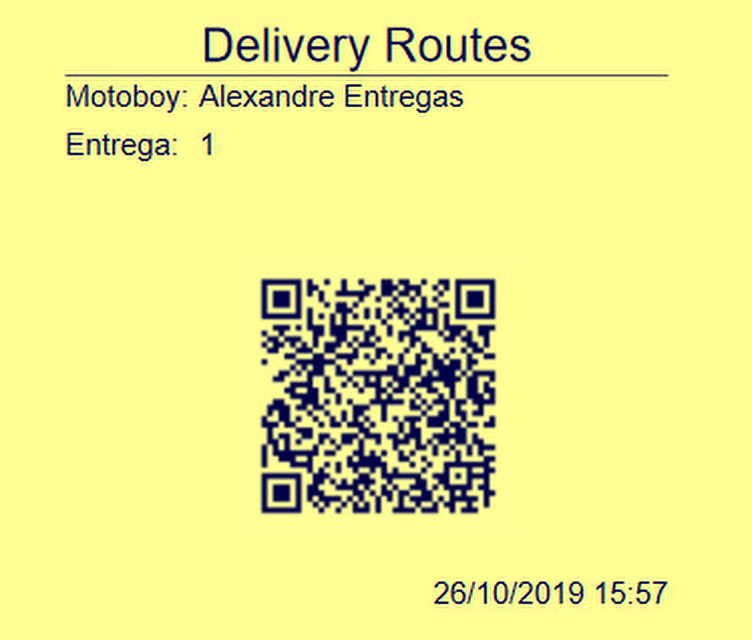
\includegraphics[width=0.4\textwidth]{./dados/figuras/fig24}
    \fonte{Autor}
    \label{fig:drCupom}
\end{figure}

\begin{figure}[H]
    \centering
    \caption{Delivery Routes - Fluxo do pedido}
    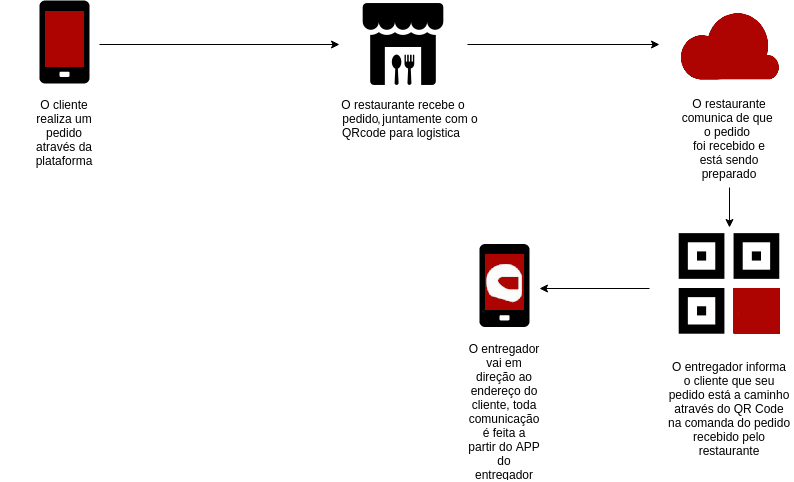
\includegraphics[width=0.85\textwidth]{./dados/figuras/fig25}
    \fonte{Adaptada de \citeonline{iFood}}
    \label{fig:drFluxoPedido}
\end{figure}

Neste cenário, ao ler o código QR impresso na comanda o motoboy é direcionado para a rota: \textit{/deliveries/{id}/dispatched} (\autoref{alg:funcDispatched}), alterando seu status para \textit{DISPATCHED} e executando uma nova rota: \textit{/deliveries/{id}/view}, onde o parâmetro solicitado para ambas é o código da entrega.

\begin{lstlisting}[caption={Delivery Routes - Função de despacho da entrega}, style=htmlcssjs, label=alg:funcDispatched]
public function dispatched($id) {
    $delivery = Delivery::find($id);
    $delivery->update(['status' => 'DISPATCHED']);
    return view('deliveries.view', compact('delivery'));
}
\end{lstlisting}

Logo após o despacho da entrega, é apresentada na tela no \textit{smartphone} do motoboy a representação, distância e tempo de deslocamento do percurso que deve ser percorrido na entrega desejada (\autoref{fig:drRotaEntregaInicio} e \autoref{fig:drRotaEntrega}).

\begin{figure}[H]
    \centering
    \caption{Delivery Routes - Despacho da entrega}
    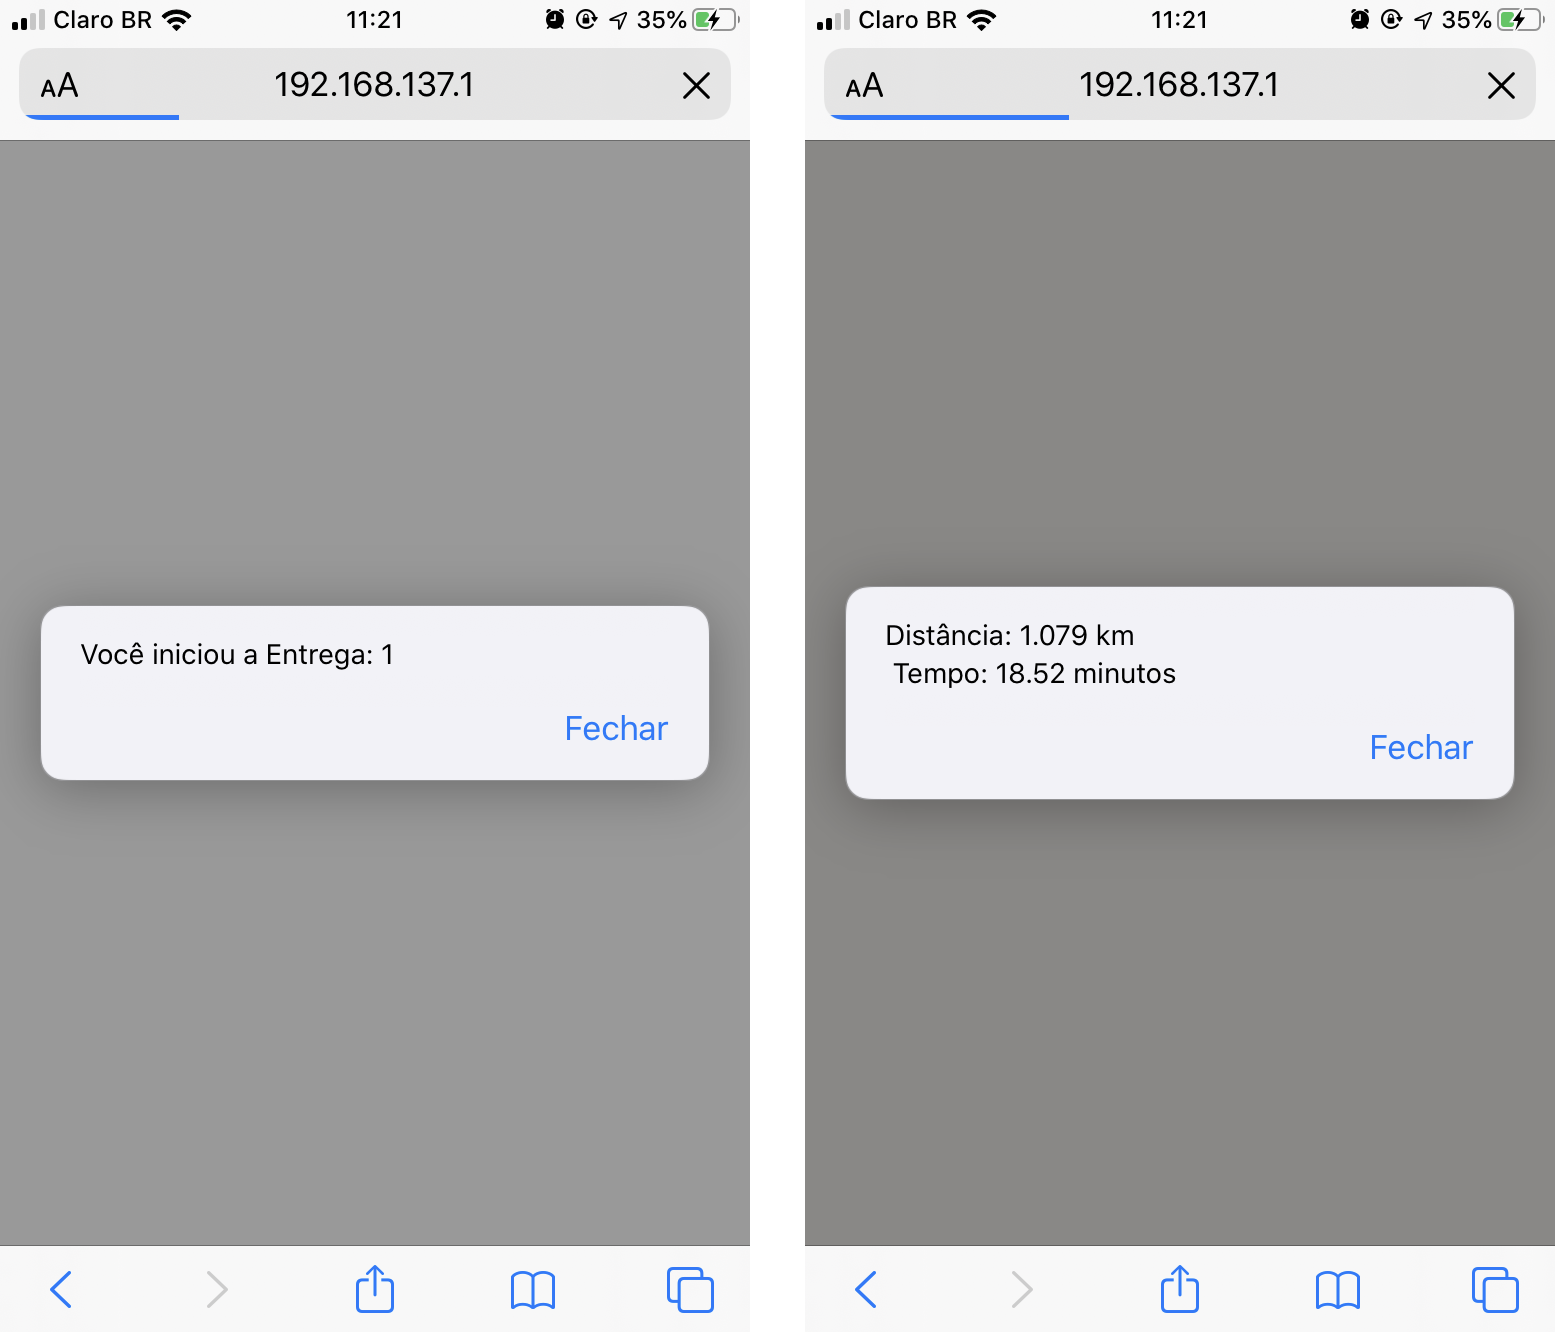
\includegraphics[width=0.9\textwidth]{./dados/figuras/fig28}
    \fonte{Autor}
    \label{fig:drRotaEntregaInicio}
\end{figure}

\newpage
\begin{figure}[H]
    \centering
    \caption{Delivery Routes - Mapa da entrega}
    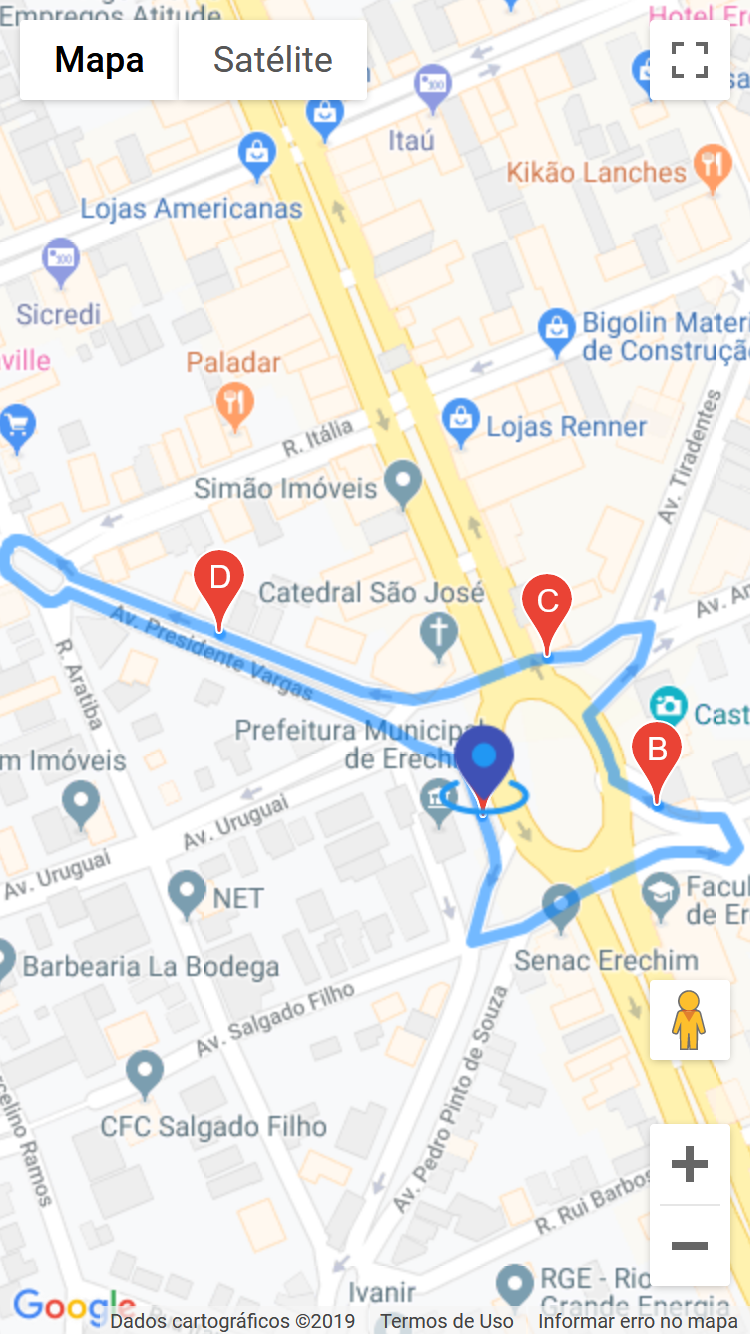
\includegraphics[width=0.8\textwidth]{./dados/figuras/fig27}
    \fonte{Autor}
    \label{fig:drRotaEntrega}
\end{figure}

\newpage
Para obter a rota entre dois pontos e exibi-la no mapa, é necessário utilizar o serviço da Google Directions API. Lendo a sua documentação, verificou-se necessário a implementação das classes \textit{google.maps.DirectionsService} e o \textit{google.maps.DirectionsRenderer}.

Começando pelo \textit{DirectionsService}, o seu funcionamento é bem simples. Basta informar um objeto \textit{google.maps.DirectionsRequest}, o qual irá conter o ponto de origem e destino (\autoref{alg:currentPosition}), e o meio de transporte (carro, a pé, bicicleta ou transporte público), que ele irá retornar um objeto \textit{google.maps.DirectionsResult}, o qual contém as informações da rota, e o \textit{google.maps.DirectionsStatus}, que por sua vez define o estado final da requisição. Ele pode indicar sucesso (\textit{OK}), sem resultados (\textit{ZERO\_RESULTS}), erro (\textit{INVALID\_REQUEST} ou \textit{REQUEST\_DENIED}), etc.

\begin{lstlisting}[caption={Delivery Routes - Função de localização do usuário}, style=htmlcssjs, label=alg:currentPosition]
navigator.geolocation.getCurrentPosition(position);
function success(position) {
    currentPosition = new google.maps.LatLng(position.coords.latitude, position.coords.longitude);
};
\end{lstlisting}

Para adicionar os pontos de parada durante a rota, adquiridos através da rota: \textit{/delivering/{id}} (\autoref{alg:pedidosEntrega}), que retorna todos os pedidos da entrega solicitada, é preciso informar uma lista de objetos \textit{google.maps.DirectionsWaypoint} (\autoref{alg:waypoints}), que são alguns pontos pré-definidos no meio do trajeto no objeto \textit{DirectionsRequest} antes de passá-lo para o \textit{directionsService.route}.

\begin{lstlisting}[caption={Delivery Routes - Route pedidos da entrega}, style=htmlcssjs, label=alg:pedidosEntrega]
Route::get('/delivering/{id}', function ($delivery_id) {
    return new OrdersResource(DB::table('orders')
    ->leftJoin('deliveries_orders', 'orders.id', '=', 
    'deliveries_orders.order_id')
    ->where('deliveries_orders.delivery_id', $delivery_id)->get());
});
\end{lstlisting}

\begin{lstlisting}[caption={Delivery Routes - Preenchimento dos pontos de parada}, style=htmlcssjs, label=alg:waypoints]
$.getJSON(json, function(pontos) {
    $.each(pontos.data, function(index, ponto) {
        waypoints[position] = {
            'location': new google.maps.LatLng(ponto.latitude, ponto.longitude)
        };
    });
});
\end{lstlisting}

\newpage
Já o \textit{DirectionsRenderer}, basicamente, fica responsável por renderizar o resultado fornecido pelo \textit{DirectionsService} (\autoref{alg:directionsService}).

\begin{lstlisting}[caption={Delivery Routes - Requisição de renderização do mapa}, style=htmlcssjs, label=alg:directionsService]
var request = {
    origin: currentPosition,
    waypoints: waypoints,
    destination: currentPosition,
    travelMode: google.maps.TravelMode.DRIVING
};

directionsService.route(request, function(result, status) {
    if (status == google.maps.DirectionsStatus.OK) {
        directionsDisplay.setDirections(result);
    }
});
\end{lstlisting}

O cálculo de distância e tempo (\autoref{alg:computeTotalDistance}), exibido na \autoref{fig:drRotaEntregaInicio}, é a última etapa. Nele é computado o tempo de deslocamento entre os pontos e também o tempo dos trâmites de entrega do produto para o cliente final, estimado em 5 minutos cada.

\begin{lstlisting}[caption={Delivery Routes - Função de cálculo do deslocamento}, style=htmlcssjs, label=alg:computeTotalDistance]
function computeTotalDistance(result) {
    var totalDist = 0;
    var totalTime = -300; // retorno
    var myroute = result.routes[0];
    for (i = 0; i < myroute.legs.length; i++) {
        totalDist += myroute.legs[i].distance.value;
        totalTime += myroute.legs[i].duration.value;
        totalTime += 300;
    }
}
\end{lstlisting}

A maioria dos produtos da Google são pagos, porém há um crédito (200 dólares para uso mensal gratuito, que condizem com até 28 mil carregamentos no valor de 7 dólares por milhar) disponível no momento da requisição dos serviços, que vai sendo debitado na medida que é requisitado. Não é cobrado valor algum até que esse crédito seja totalmente utilizado. Ele pode ser usado no Maps, no Routes ou no Places. Para fins de uso e cobrança, é necessário uma chave da API JavaScript do Google Maps. A chave da API é um identificador exclusivo usado para autenticar solicitações associadas ao projeto.